\chapter{Ontogeny of circadian rhythms and synchrony in the suprachiasmatic nucleus}
\blfootnote{Major portions of this chapter appear as V.~Carmona-Alcocer, J.H.~Abel, T.C.~Sun, L.R.~Petzold, F.J.~Doyle~III, C.L.~Simms, and E.D. Herzog, ``Ontogeny of circadian rhythms and synchrony in the suprachiasmatic nucleus,'' Journal of Neuroscience, accepted. All statistical and mathematical analysis and modeling was performed by J.H. Abel. All experimental work was performed by members of the Herzog lab, primarily V.~Carmona-Alcocer. This journal article, and thus a major portion of this chapter, was written collaboratively with V.~Carmona-Alcocer and E.D. Herzog.
%copyright info email sent: http://www.jneurosci.org/sites/default/files/files/permissions_policy.pdf
}

\section{Introduction}
How and when hypothalamic circadian rhythms arise during development is not known.
More precisely, it has not been established when cell-autonomous circadian rhtyhms in the SCN arise, and how and when the network establishing intercellular synchrony first appears.
Studies of whole-SCN circadian development do not make the distinction between single-cell and whole-tissue oscillation, further obscuring the development of the SCN network, which is necessary for synchronous oscillation.

In mice, it is well-established that neurogenesis of the SCN occurs between embryonic days 10-15 (termed E10-15, where E1 is the day when a vaginal plug is detectable), peaking between E12-14 and forming from ventrolateral to dorsomedial \cite{Shimada1973,  Kabrita2008, Shimogori2010}.
It is further known that a variety of transcription factors are expressed during differentiation of the SCN (e.g.\ \textit{Lhx1}, \textit{Shh}, \textit{Six3}, \textit{Six6}) \cite{Shimogori2010, VanDunk2011, Clark2013, Bedont2014}.
Development also continues postnatally, and synaptogenesis has been found to occur primarily after birth \cite{Moore1989, Shimogori2010}.
Although the SCN continues to develop after birth, numerous studies in rats have shown that circadian rhythms in fetal metabolism, and circadian spontaneous electrical activity and clock gene expression within fetal SCN, begin before birth \cite{reppert1983maternal, reppert1984suprachiasmatic, Shibata1987, Sladek2004, Kovacikova2006, Houdek2014}.
Studies of mice have yielded similar results to rat studies, with detectable fetal daily rhythms in \textit{Per1} transcript levels at E17, and PER1 and PER2 proteins by E18 \textit{in vivo} \cite{Shimomura2001, Ansari2009}.
\textit{In vitro} studies of SCN explants have found circadian expression of the PERIOD2::LUCIFERASE (\textit{Per2}$^{Luc}$) bioluminescent reporter in the whole SCN as early as E13 \cite{Landgraf2015} or E15 \cite{Wreschnig2014}.
Still, it remains unclear if these oscillations are self-sustaining and spontaneously synchronizing as in the mature SCN, or driven or coordinated by the circadian oscillator of the mother.

In the mature SCN, neurons exchange electrical and neurotransmitter signals to maintain identical periods and consistent phase relationships \cite{Mohawk2011, Herzog2015, Evans2016}. 
Among these signals, vasoactive intestinal peptide (VIP) has attracted significant attention for its essential role in SCN synchrony \cite{Aton2005}.
The absence of VIP or its receptor, VIPR2, reduces synchrony between neurons and consequently eliminates many daily rhythms, while exogenous application of VIP is able to restore synchrony to the VIP$^{-/-}$ SCN \textit{in vitro} \cite{Harmar2002, Colwell2003, Aton2005, Maywood2006, Ciarleglio2009}.
It remains unknown when VIP is first expressed in the SCN, and whether its role in the fetal SCN is identical to that in the adult \cite{Wang2014, Ono2016}.
For example, GABA, another neurotransmitter expressed in the SCN, is known to have very different effects in the fetal brain because of differing chloride potentials \cite{fain1999}.
In this chapter, we used the \textit{Per2}$^{Luc}$ bioluminescent reporter to study the onset of circadian rhythms in the SCN at at near-single-cell scale.
We sought to identify the onset of self-sustained genetic circadian oscillations in individual cells, spontaneous synchronization within the explanted SCN, and other markers of the mature SCN including expression of neurotransmitters with circadian relevance.

\section{Materials and methods}

\subsection*{Animals}
All mice were maintained on a C57BL/6JN background (WT) and housed in a 7am-7pm light-dark cycle in the Danforth Animal Facility at Washington University.
The $Per2^{Luc}$ mouse line was generated by replacing the endogenous mouse \textit{Period2} gene locus with a $Per2^{Luc}$ reporter construct \cite{Yoo2004}.
For immunochemistry, we compared male and female homozygous $Per2^{Luc}$ pups to $Vip^{-/-}$ and $Vipr2^{-/-}$ pups as negative controls.
Vaginal plugs confirmed overnight mating of each female.
We designated the morning after mating as embryonic day 0.5 (E0.5) and the day of birth as postnatal age 0 (P0).
All procedures were approved by the Animal Care and Use Committee of Washington University and followed National Institutes of Health guidelines.

\subsection*{Cultures and bioluminescence recording}
Pregnant mice were euthanized with CO$_2$ and cervical dislocation and their embryos dissected into 4$^\circ$C Hanks Buffered Saline Solution (Sigma).
All surgeries started at 1:00 PM (Zeitgeber Time, ZT 06).
We recorded bioluminescence from 300 $\mu$m coronal SCN slices from fetal (E13.5-E15.5 and E17.5) and postnatal (P2) homozygous $Per2^{Luc}$ mice \cite{Landgraf2015}.
Briefly, brains were embedded in a block of 4\% low-melting agarose and prepared with a vibraslicer.
SCN were dissected with scalpels from sections of the ventral hypothalamus and placed on 0.4 mm membrane inserts (Millipore) in sealed 35 mm Petri dishes (BD Biosciences) with 1 mL Dulbecco's Modified Eagle Medium (Sigma, pH 7.2), supplemented with 25 U/mL penicillin, 25 $\mu$g/mL streptomycin (Invitrogen), 10 mM HEPES (Sigma), 2\% B27 (Invitrogen), 0.35 g/L NaHCO3 (Sigma) and 0.15 mM beetle luciferin (Promega).
SCN explants were transferred to a light-tight incubator at 36$^\circ$C (Onyx, Stanford Photonics).
We collected images (XR Mega-10AW camera, Stanford Photonics) every 6 min (6 sec exposure) and then summed every 10 frames with ImageJ software (http://rsbweb.nih.gov/ij) to provide one image every hour.
We applied adjacent frame minimization to each movie to filter out bright noise caused by the camera or cosmic rays.

\subsection*{Data analysis}
We analyzed the $Per2^{Luc}$ rhythms of the developing SCN at the level of the whole tissue and with 30 $\mu$m (pixel) resolution.
The statistical analysis for each experiment is described in detail in its respective section.
We assessed rhythms measured as the integrated intensity of the SCN tissue with cosinor analysis (software from B. Meier and A. Kramer).
We performed a pixel-based analysis of the same SCN movies.
We excluded movies if the corners of the SCN slice moved (3 slices excluded at each of E15.5, 17.5 and P2).
We measured periodicity of each pixel (1 px = 900 $\mu$m$^2$) and defined pixels as circadian if they had a dominant period between 18-32h with $P < 0.05$ by Lomb-Scargle periodogram analysis \cite{Ruf1999}; or a correlation coefficient greater than 0.6 in cosinor analysis.
Because the two methods yielded 90 $\pm$ 0.02\% (mean $\pm$ S.E.; n=30 brains) agreement in pixel classification, we reported results from the periodogram analysis only.
The cycle-to-cycle variability in $Per2^{Luc}$ was evaluated by detrending rhythmic cells with a discrete wavelet transform \cite{Leise2011} keeping only detail coefficients between 16-32h, and measuring the interpeak distance (h) of each cycle.
We evaluated the synchrony index using the Kuramato method \cite{kuramoto1984}, with instantaneous phase calculated using a Hilbert transform of the detrended and denoised data.

A radial distribution of mean peak times was constructed for each SCN to identify the presence of core-shell structure.
The time of the initial peak for each pixel was calculated following detrending.
A radial distribution of peak times was constructed by binning individual cell peaks based on radial distance from a reference point in the left ventrolateral SCN.
A null distribution of radial peak times was calculated by bootstrapping: reassigning peak time values at random to pixels within each SCN and recalculating the radial distribution using 10,000 bootstrap runs.
An SCN was determined to have core-shell structure if the radial peak time distribution showed significant (P < 0.05) peaks for the shell region (early-peaking, middle distances) and at least one core region (late-peaking, near and far distances). 

\subsection*{Software}
Data analysis was performed in the Python language, using packages scipy and numpy \cite{jones2014scipy}, PyWavelets, Statsmodels \cite{Seabold2010}, and Matplotlib \cite{Hunter2007}.
Parallelization of data processing was achieved via iPython \cite{Perez2007}.

\subsection*{Immunocytochemistry}
Brains of mice from ages E13.5-E17.5, P0 and P2 were removed and fixed in 4\% paraformaldehyde in phosphate buffered saline (PBS) overnight at 4$^\circ$C.
We transferred them to 30\% sucrose in PBS for 24 h at 4$^\circ$C and sectioned in 30 $\mu$m thick coronal slices onto microscope slides.
The sections were incubated for 1 h at 4$^\circ$C in a blocking solution (10\% not fat dry milk, 10\% bovine serum albumin and 0.3\% TritonX-100 in PBS) and then for 48 h at 4$^\circ$C in an anti-VIP (1:1000, Imunostar) or anti-VPAC2R (1:1000, Abcam) rabbit polyclonal antibody diluted in 3\% BSA and 0.35\% TritonX-100 in PBS.
After washing in PBS, the slides next were incubated at room temperature in a biotinylated goat anti-rabbit IgG (1:200; Vector) for 2 h and then ABC solution (1:200; Vectastain Elite ABC Kit, Vector) for 2 h.
Finally, we incubated each slide in 50 mM Tris-HCl using 3,3-diaminobenzidine kit (Sigma).
After each step, we rinsed 3 times for 15 minutes in PBS.
Mounted sections were dehydrated through a series of ethanol and xylene washes.
Slides were imaged (NanoZoomer microscope, Leica) and the integrated optical density of the SCN was measured using ImageJ software \cite{Schneider2012}.

\subsection*{Drug treatments} 
All drugs were diluted in deionized water and they remained in the recording medium throughout the entire recording without further medium changes.
VIP antagonist (200nM PG-99465) provided by Dr.\ P.\ Robberecht \cite{Cutler2003}, GABA antagonist (100 $\mu$M Gabazine, TROCRIS), MEC (10 $\mu$M Meclofenamic acid, SIGMA), or TTX (2.5 $\mu$M tetrodotoxin).


\section{Results}

\subsection*{SCN cells become reliable circadian oscillators after E14.5}
\begin{figure}[p]
    \begin{center}
        \includegraphics[width=3.3in]{chap4/figures/Figure1.png}
    \end{center}
    \caption{\label{fig:vc1} {\small Circadian rhythms in the SCN during development.  Long-term, real-time recordings of PER2 expression from SCN harvested after E14.5 showed reliable circadian periods between 18-32h. (\textbf{A}) Representative records of $Per2^{Luc}$ bioluminescence from SCN starting on the day they were explanted. Note the weak circadian oscillations that were found in some E14.5 SCN. Insets show images of two representative SCN from each age. Some SCN harvested at E13.5 expressed $Per2^{Luc}$ above the SCN region along the ventricular zone of dorsal hypothalamus (blue arrow head, n=5/8). All others harvested at this age and older reliably expressed high levels of PER2 in the bilateral SCN. Scale bar = 10 px = 300 $\mu$m. (\textbf{B}) Nearly all SCN expressed significant circadian rhythms when harvested on or after E15.5 (Upper panel), with periods close to 24 h (mean ± SEM; Middle panel) and durations of daily $Per2^{Luc}$ expression above the mean close to 12 h (alpha; mean $\pm$ SEM, Lower panel; *P < 0.05, one-way ANOVA, Tukey's HSD). Note, 8 slices were examined at E13.5, however, we excluded 5 because they did not express detectable PER2 in the SCN region.}
    }
\end{figure}

Recent in vitro studies have demonstrated the presence of circadian rhythms in PER2 expression in whole SCN explants at E13 \cite{Landgraf2015} or E15 \cite{Wreschnig2014}, around the times of peak or completed neurogenesis, respectively.
To test if cell-autonomous oscillations appear prior to tissue-level rhythms, we imaged bioluminescence in fetal $Per2^{Luc}$/$Per2^{Luc}$ SCN slices.
SCN explanted at E13.5 displayed no tissue-level circadian rhythms (n = 8 SCN from 2 litters; Fig. 
\ref{fig:vc1}).
At this stage, the ventricular zone of dorsal hypothalamus expressed high levels of PER2, sometimes in a circadian pattern (n = 2 of the 8 slices), but the bilateral SCN region had low to no PER2 expression and no circadian rhythms.
In contrast, all tissues explanted on E14.5 or later displayed bilateral $Per2^{Luc}$ expression in the ventral hypothalamus, corresponding to the SCN.
By E14.5, 45\% of SCN were circadian (5 of 11 SCN from 4 litters).
Notably, some E14.5 explants (n = 4 of 11) also displayed no rhythmic $Per2^{Luc}$ expression outside the SCN in the ventricular zone of the dorsal hypothalamus.
By E15.5, no hypothalamic explants showed high PER2 expression outside the SCN region and nearly all SCN were circadian (n = 11 of 12 E15 SCN from 4 litters, 7 of 7 E17 SCN from 2 litters and 5 of 6 P2 SCN from 1 litter).
We conclude that PER2 expression is localized to the SCN and becomes circadian on E14.5.

\begin{figure}[p]
    \begin{center}
        \includegraphics[width=6.5in]{chap4/figures/Figure2abcd_vc.png}
    \end{center}
    \caption{\label{fig:vc2} Embryonic SCN cells express PER2 rhythmically beginning around E14.5 in vitro. (\textbf{A}) Heat maps of two SCN explanted at each developmental stage show circadian pixels based on Lomb-Scargle periodogram (power above P < 0.05) and Cosinor analysis (correlation coefficient greater than 0.6). We therefore report results only from periodogram analyses for simplicity. (\textbf{B}) Representative Per2Luc bioluminescence images of the same SCN explants (1 h integration, 2 x 2 binning). Scale bar = 10 px = 300 $µ$m. (\textbf{C}) Representative Per2Luc bioluminescence recordings from single rhythmic pixels from SCN cultured at different embryonic stages. Note the competence of the E15.5 SCN to generate and sustain circadian rhythms in PER2 protein expression. (\textbf{D}) The fraction of circadian pixels in each SCN (mean $\pm$ SEM,) was higher for explants at E15.5 and older (*P < 0.05, one-way ANOVA, Tukey's Honestly Significant Difference (HSD), n=at least 3 SCN at each age where age is reported as days post mating, E0.5, and post birth, E20.5=P0). 
    }
\end{figure}


We next developed methods to culture and image the embryonic SCN for at least 5 days.
From these movies, we quantified local circadian rhythms where each pixel included approximately 10 or fewer cells (Fig. 
\ref{fig:vc2}A-B).
We found the fraction of circadian pixels (cells) increased approximately 7-fold from E14.5 (Fig. 
\ref{fig:vc2}C-D; 0.10 $\pm$ 0.07, mean $\pm$ SEM; n=11 SCN from 4 litters) to E15.5 (0.72 $\pm$ 0.11; n = 9 SCN from 4 litters; *P < 0.05, one-way Kruskal-Wallis H(3)=10.62, with posthoc Tukey's Honestly Significant Difference).
Nearly all regions were circadian in SCN explanted on E17.5 (0.96 $\pm$ 0.03; n = 4 SCN from 2 litters) and postnatal day 2 (P2, 0.97 $\pm$ 0.02; n = 3 SCN from 1 litter).  
The developmental increase in the number of circadian regions correlated with an increase in circadian period in the SCN (Fig. 
\ref{fig:vc3}A-B).
We conclude that a small number of SCN cells initiate endogenous circadian rhythmicity by E14.5, and by E15.5 SCN cells are rhythmic throughout the SCN.

To determine the precision of SCN rhythms during development, we measured the cycle-to-cycle difference in period for each pixel within the fetal SCN over three days of the recording. Interestingly the increase in the number of circadian oscillators correlated with an increase in circadian precision (Fig. 
\ref{fig:vc3}C-D), suggesting that addition of circadian cells lengthens and stabilizes period in the SCN.

\begin{figure}[p]
    \begin{center}
        \includegraphics[width=6.5in]{chap4/figures/Figure3_vc.png}
    \end{center}
    \caption{\label{fig:vc3} Circadian period and precision of SCN cells increased with development. (\textbf{A}) Heat maps from representative SCN show the mean period over 5 days of recording. (\textbf{B}) The fraction of rhythmic pixels correlated with an increase in the mean SCN period (Least-squares linear regression P = 0.00019, Pearson's r = 0.74. SCN with fewer than 5 circadian pixels were considered arrhythmic and excluded from this analysis.  E14.5: diamonds, n=6 of 11, E15.5: circles, n=9 of 9, E17.5: triangles, n=4 of 4, P2: squares, n=3 of 3).  (\textbf{C}) Representative mean cycle-to-cycle variability heat maps show the increase in circadian precision with age. Scale bar = 150 $\mu$m. (\textbf{D}) The average variability of the daily period across all rhythmic pixels within each isolated SCN inversely correlated with the fraction of circadian cells (least-squares linear regression P = 0.0006, Pearson's r = -0.70; symbols as in B), SCN with fewer than 5 circadian pixels were considered arrhythmic and excluded from this analysis.
    }
\end{figure}

\begin{figure}[p]
    \begin{center}
        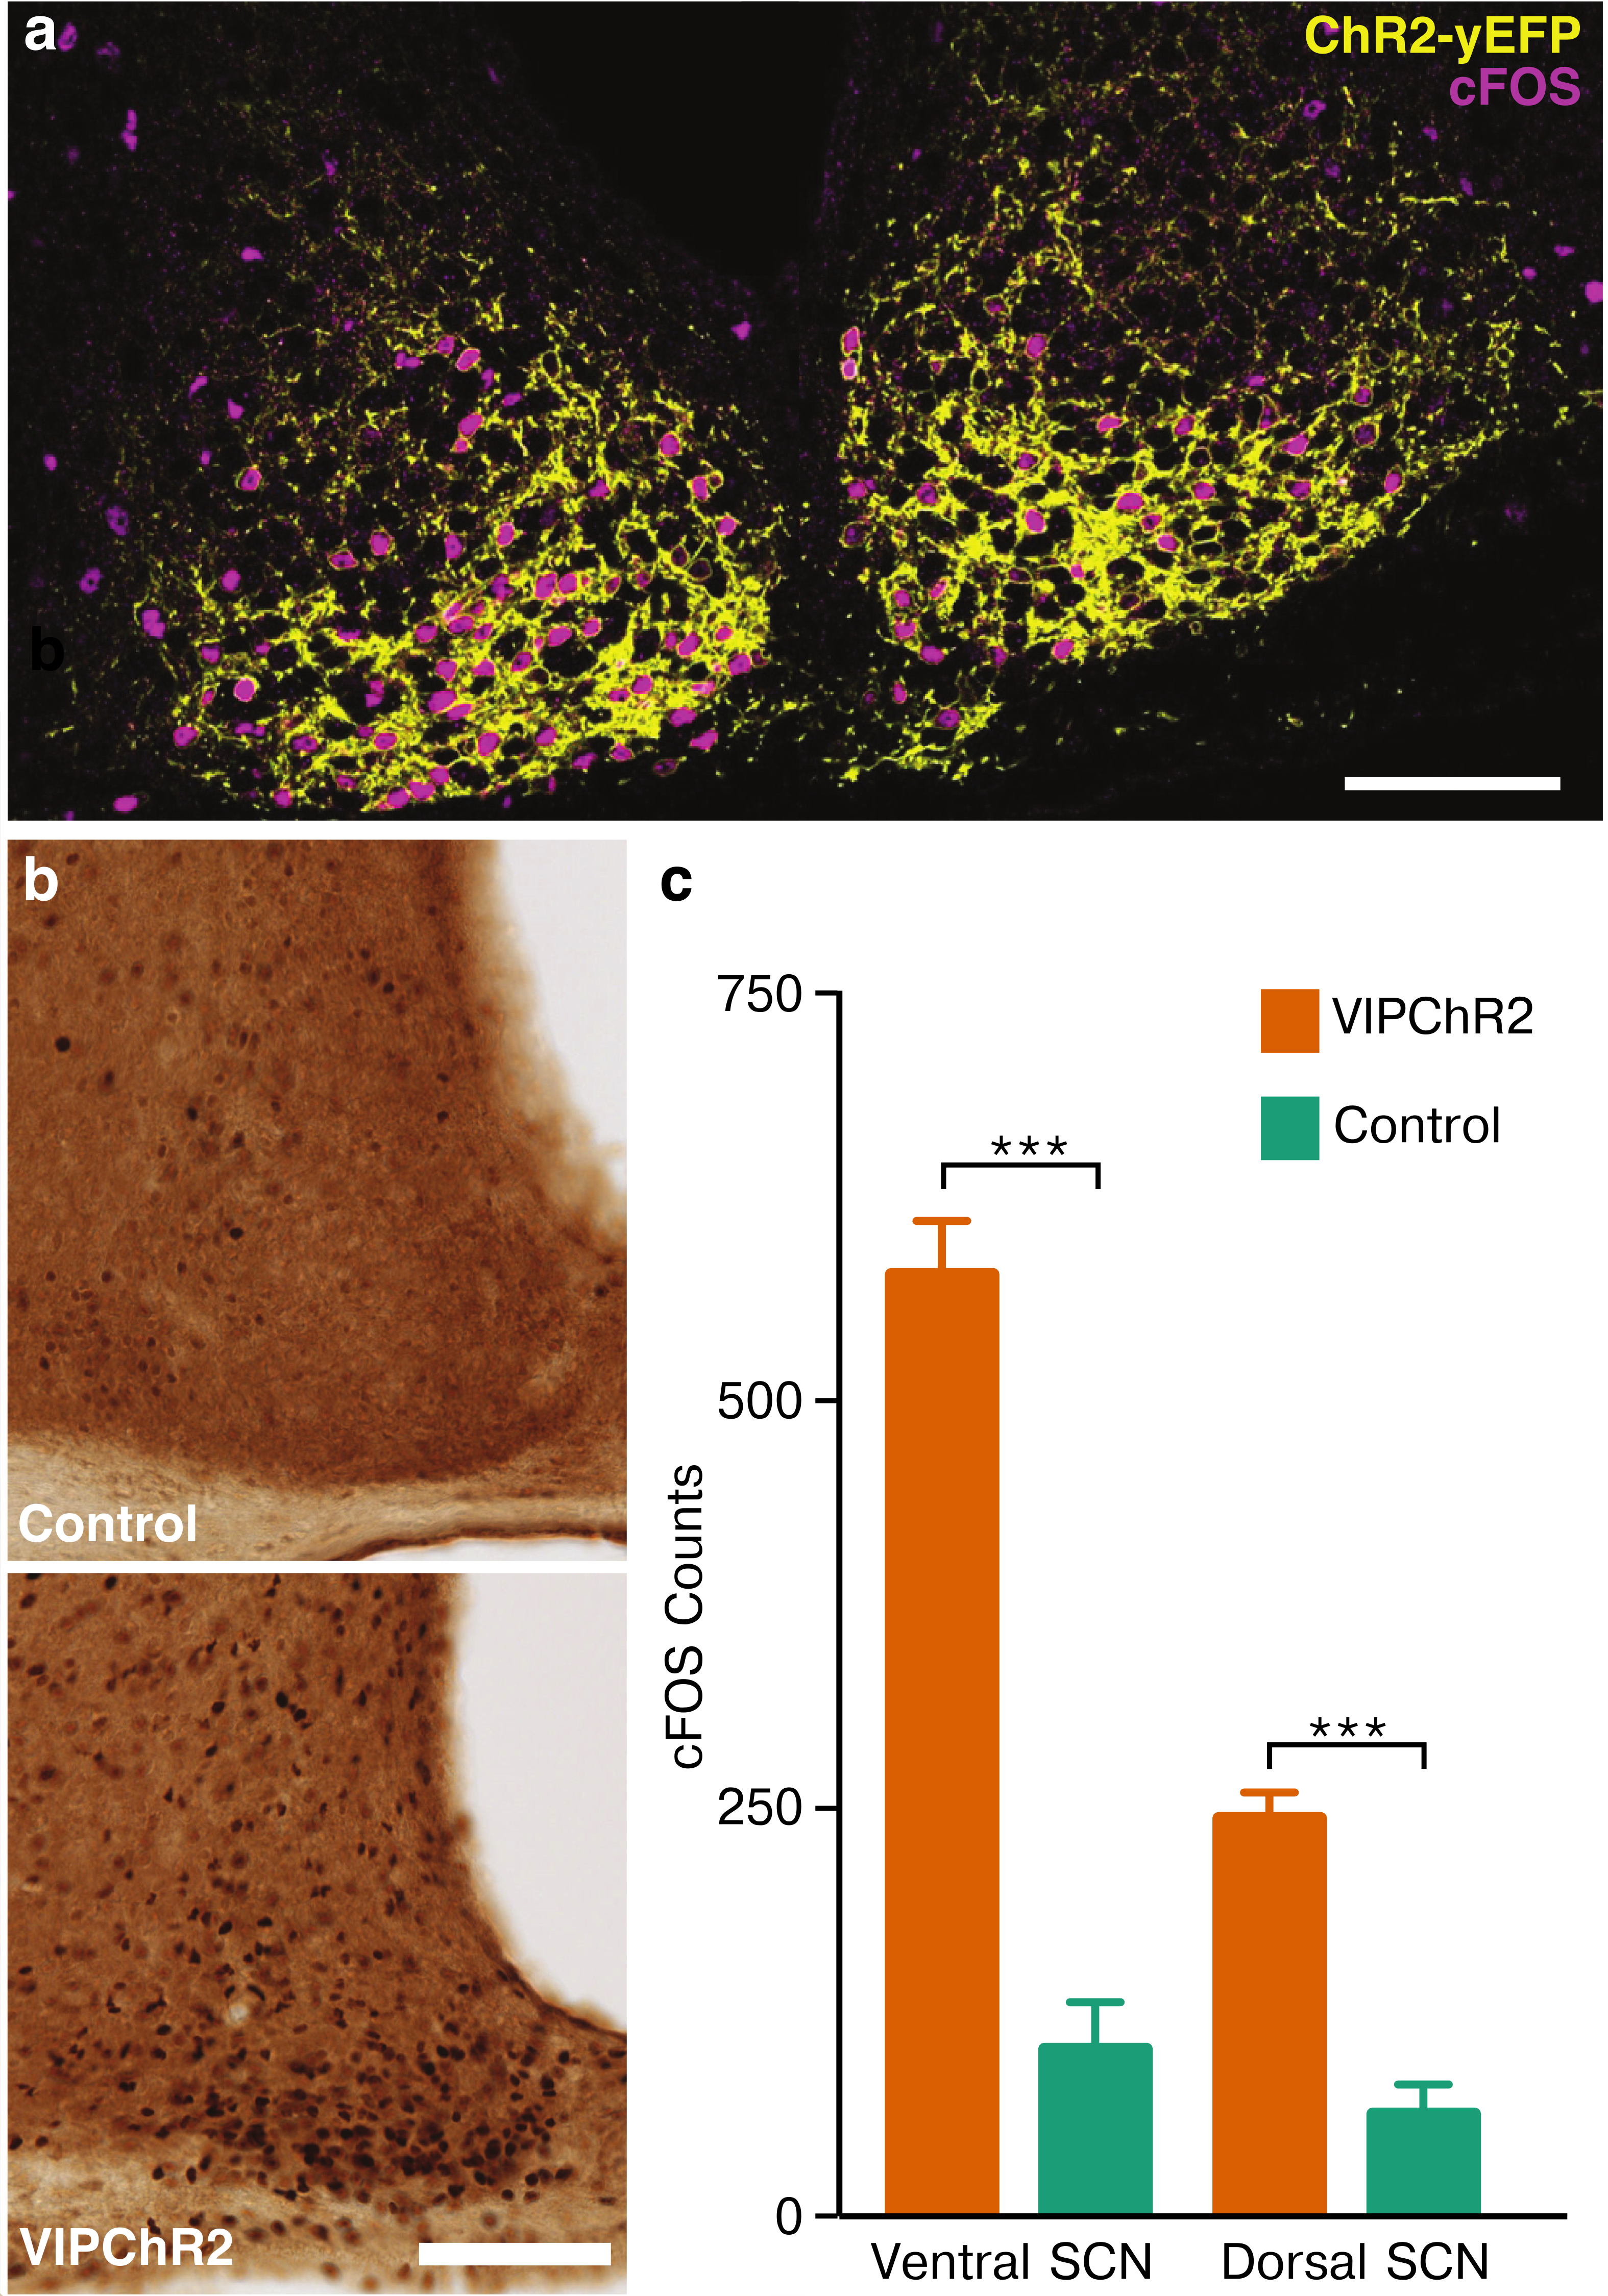
\includegraphics[width=3.5in]{chap4/figures/Figure4.png}
    \end{center}
    \caption{\label{fig:vc4} The phase wave of PER2 expression in the SCN appeared only after birth. (\textbf{A}) Heat maps of the time of peak PER2 expression across representative SCN. Note the dorsal-to-ventral distribution across the cells of the P2 SCN. Scale bar = 300 $\mu$m. (\textbf{B}) Radial distribution of peak times revealed a core-shell structure in the P2, but not younger, SCN explants. We compared the average differences in the times of peak PER2 expression as a function of distance from the ventral margin of each SCN with a null distribution of randomly shuffled peak times (shaded area=95\% CI for mean peak time calculated from 10,000 resamples). At P2, PER2 peaked significantly later in the ventral core than the dorsal shell, as seen in this representative example. 
    }
\end{figure}


\subsection*{The phase wave typical of adult SCN appears around P2}


In adults, PER2 expression progresses as a daily wave from dorsal to ventral across the SCN \cite{Yan2002, Quintero2003, Yamaguchi2003, Evans2011}.
We examined when this spatiotemporal patterning of circadian expression arises in the SCN. To do so, we identified the times of daily peak PER2 in each pixel of the SCN and tested for spatial organization of expression.
We found reliable daily waves of PER2 from the dorsal to ventral SCN by P2, but not at earlier developmental stages (Fig. 
\ref{fig:vc4}).
We conclude that phase relationships among SCN cells continue to mature after birth.



\subsection*{Onset of synchrony and intercellular communication within the SCN}

Synchronous circadian oscillations in the SCN are required to coordinate daily rhythms in behavior \cite{Schwartz1987, Aton2005, Ohta2005}.
To test how synchrony develops, we measured the cycle-to-cycle variability in period length and the synchrony index (SI), a quantity that ranges from 1.0 (all oscillators peak together) to 0.0 (all cells peak at uniformly different times of day) from five days of recording.
We found that synchrony tends to increase between E14.5 (Fig. 
\ref{fig:vc5}; SI = 0.80$\pm$0.5, n = 6 SCN) and E15.5 (SI = 0.87$\pm$0.05, n = 9 SCN) reaching a maximum around E17.5 (SI = 0.91$\pm$0.02, n = 4) and P2 (SI = 0.94$\pm$0.02, n = 3 SCN (one unilateral due to changes during recording between halves)). 
Although there is no significant differences in the SI between ages, SI was positively correlated with the fraction of SCN cells displaying daily rhythms, indicating that intercellular synchrony is developed simultaneously with increased endogenously generated cellular oscillation (Fig. 
\ref{fig:vc5}C). 



We next examined the signaling pathways that could enable synchronization of SCN cells starting around E15.5.
VIP signaling is necessary for coordinated circadian rhythms among SCN cells and in behavior of adult mice \cite{Harmar2002, Colwell2003, Aton2005, Maywood2006, Ciarleglio2009}.
We measured the levels of VIP, and its cognate receptor, VIPR2, by immunocytochemistry between days E14.5 and P2 (Fig. 
\ref{fig:vc6}).
We found VIP (12.5$\pm$2.3, n = 7) and VIPR2 (15.0$\pm$5.6 relative optical density (ROD), n = 6) were detectable postnatally above baseline (immunolabeling in the P2 SCN of $Vip^{-/-}$ = 2.1$\pm$0.7 ROD, n = 5 brains and $Vipr2^{-/-}$ =3.8$\pm$2.1 ROD, n = 5, mean$\pm$SEM), but not earlier stages.
To further explore this surprising result, we found that a VIP antagonist did not affect synchrony of the E15.5 SCN (Fig. 
\ref{fig:vc7}).
Consistent with prior publications, we found that addition of the VIPR2 antagonist reduced the fraction of circadian cells in the isolated adult SCN to 30\% from 84\% (n = 1 adult SCN; \cite{Cutler2003, Aton2005}.
We conclude that VIP and its receptor VIPR2 appear in the SCN after the initiation of circadian rhythms and are not required for circadian synchrony among embryonic SCN cells.

We then performed further pharmacological experiments to test if GABA and/or gap junctions, other candidate coupling mechanisms, might drive synchrony in the SCN before VIP expression begins. 
Remarkably, antagonists against either or both GABA and gap junctions did not reduce the synchrony index of the E15.5 SCN (Fig. \ref{fig:vc7}).


\begin{figure}[!p]
    \begin{center}
        \includegraphics[width=6.5in]{chap4/figures/Figure5.png}
    \end{center}
    \caption{\label{fig:vc5} The synchrony between SCN cells increased and became more stable as the fraction of circadian cells increased. (\textbf{A}) Representative traces of the synchronization index (also called the Kuramoto order parameter or Rayleigh Statistic, r) among regions within the cultured SCN at different ages. (\textbf{B}) The average synchronization index of SCN slices (mean $\pm$ SEM, 24 h excluded from either end of analysis) did not reliably increase with age, but (\textbf{C}) correlated with the fraction of circadian cells in the SCN (symbols as in prior figure, Least-squares linear regression P = 0.004, Pearson's r = 0.61, n=at least 3 SCN at each age).
    }
\end{figure}

\begin{figure}[!p]
    \begin{center}
        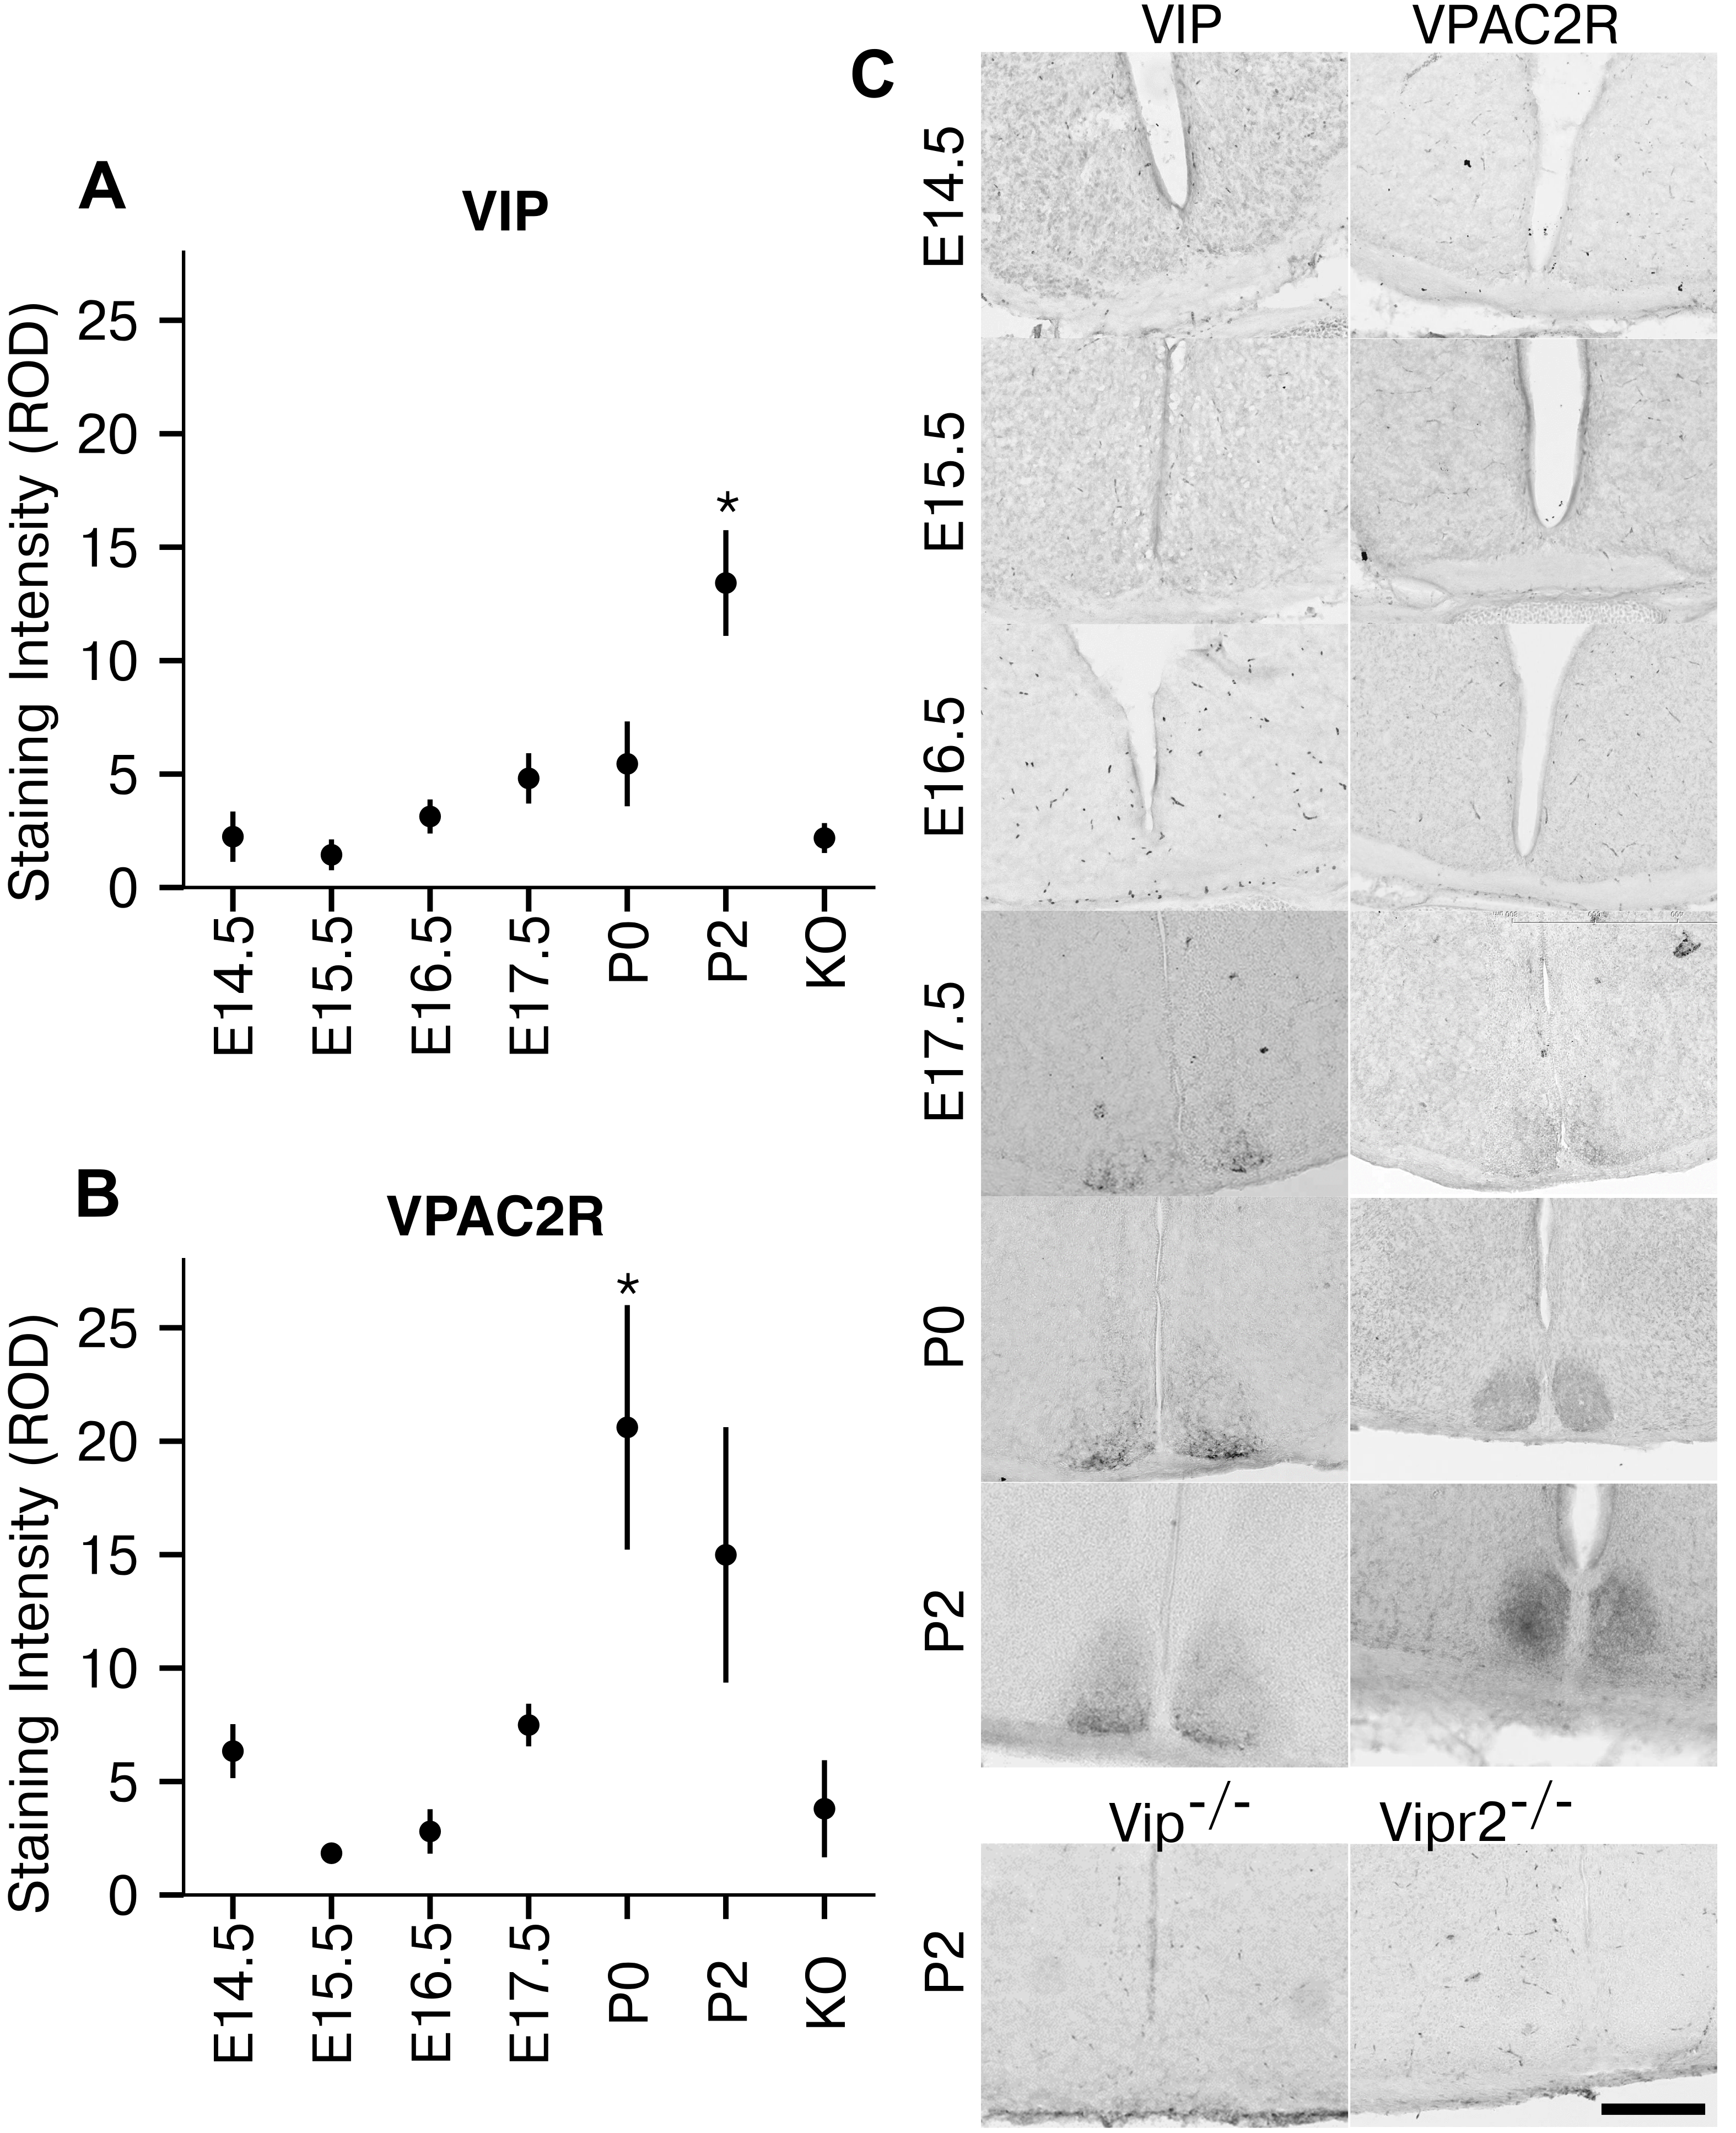
\includegraphics[width=3.5in]{chap4/figures/Figure6.png}
    \end{center}
    \caption{\label{fig:vc6} VIP and VPAC2R expression matured in the postnatal SCN. (\textbf{A}) Immunostaining intensity (Mean relative optical density $\pm$ SEM, n=9, 5, 7, 6, 7 and 7 brains at each age, respectively) of VIP in the SCN was significant by P2 compared to Vip-knockout controls (n=5, *P < 0.05, one-way ANOVA with Tukey’s HSD). (\textbf{B}) Immunostaining intensity (Mean ± SEM) of VPAC2R (n=6, 6, 5, 5, 7, and 6 brains, respectively) was significant by P0 compared to Vipr2-knockout controls (n=5, *P<0.05, one-way ANOVA with Tukey’s HSD). (\textbf{C})  Representative coronal SCN sections show the VIP (left panel) and VPAC2R (right panel) immunoreactivity at different ages. Scale bar = 200 $\mu$m.
    }
\end{figure}


\begin{figure}[!p]
    \begin{center}
        \includegraphics[width=6.5in]{chap4/figures/Figure7.png}
    \end{center}
    \caption{\label{fig:vc7} Antagonists of GABA or VIP signaling, gap junctions or neuronal firing did not disrupt circadian synchrony in the developing SCN. Drugs applied during the first day of culture of E15.5 SCN explants did not change (\textbf{A}) the fraction of pixels with circadian \textit{Per2}$^{Luc}$ (grey bars show the means across all SCN recorded at each developmental stage), or (\textbf{B}) the mean sync index over the 5 days of recording. (\textbf{C}) The synchronization index within a representative cultured E15.5 SCN treated with Veh (Vehicle), Gz (100 $\mu$M Gabazine), MEC (10 $\mu$M Meclofenamic acid), VIP antagonist (200 nM PG-99465), or TTX (2.5  $\mu$M tetrodotoxin).
    }
\end{figure}

\clearpage
\section{Discussion}

Our results indicate that E15.5 is a critical time in the maturation of the SCN.
The clock gene, PER2, is first expressed on E14.5 in the SCN and approximately 10\% of these SCN cells are weakly circadian.
By E15.5, nearly all cells within the SCN show circadian oscillation in gene expression.
Previous studies have identified E15.5 as the end of neurogenesis \cite{Shimada1973, Kabrita2008, Shimogori2010}, and transcription factors Lhx1 and ROR$\alpha$ are widely expressed across the SCN \cite{VanDunk2011}.
In particular, ROR$\alpha$ deserves further study, as it is known to be a core component of the mammalian circadian oscillator.
ROR$\alpha$ is a positive regulator of \textit{Bmal1} expression \cite{Sato2004}, and \textit{Bmal1} is an essential transcription factor and activator of \textit{Per} gene expression \cite{Hastings2014, Takahashi2016}.
ROR$\alpha$ knockout adult mice showed slight behavioral abnormalities in circadian rhythms.
We therefore speculate that expression of ROR$\alpha$ or another transcription factor in the SCN at E15.5 induces the onset of autonomous circadian oscillations in SCN cells.

Consistent with a prior publication \cite{Landgraf2015}, we found no evidence that development occurs \textit{in vitro}: on average we did not find increases in the number of oscillatory cells or SCN-wide synchrony as a recording progressed.
For example, SCN explanted on 13.5 were arrhythmic and did not show an increase in the fraction of rhythmic pixels over the course of the experiment.
SCN isolated at E14.5 or E15.5 similarly did not show changes in the amplitude, period, variability or fraction of circadian cells during 7-day recording.
Although we cannot rule out that arrhythmic, fetal SCN cells cultured longer than 7 days might develop daily cycling, our results indicate that the transition from arrhythmic to circadian is rapid and likely requires signals from outside the fetal SCN.
Other studies have found that stem cells exhibit autonomous oscillations after inducing differentiation with retinoic acid \cite{Yagita2010, Inada2014}.
Our result suggest that this signal, if it indeed initiates oscillation, does not originate spontaneously within the SCN.

Interestingly, we found that PER2 was first expressed outside the SCN.
At E14.5, extra-SCN PER2 expression was high and occasionally circadian, but was nearly completely eliminated by E15.5. 
It is not clear whether these PER2-expressing cells move into the SCN or remain in the dorsal hypothalamus while reducing their PER2 expression.
Anecdotally, it appeared that neuronal migration into the SCN region may explain this extra-SCN PER2 expression.
Further study with more rapid imaging than 1/hr would be needed to examine this possibility.
Still, rhythmic bioluminescence in these extra-SCN regions could explain the discrepancy between previous studies reporting the onset of PER2 daily oscillations in hypothalamic explants at E13 or E15 \cite{Wreschnig2014, Landgraf2015}.
The correlations between increasing fraction of rhythmic cells, increasing circadian period, and increasing period precision during this time could reflect the consequences of cell-cell communication \cite{Webb2009} or differential expression of molecular components of the circadian oscillator \cite{VanDunk2011, Ono2016}.
Together, these data support the onset of cell-autonomous circadian oscillation between E14.5 and E15.5, with intercellular communication developing shortly thereafter.

The SCN in adult mice displays a dorsal to ventral phase wave in clock gene expression \cite{Yan2002, Quintero2003, Yamaguchi2003, Evans2011a}.
Because this phase wave is not a fixed property  (e.g., it can adopt a different pattern after a temperature manipulation \textit{in vitro}) \cite{Jeong2016}, it is important to consider whether the results from the isolated SCN reflect its \textit{in vivo} circadian properties, or are simply reflective of its environment.
Our results indicate that under the constant conditions we employed, the SCN phase wave first appears after birth.
SCN explant procedures were performed at identical times of day, so although surgery has been shown to strongly reset circadian phase \cite{Wreschnig2014, Landgraf2015}, it is unlikely to cause spatial wave seen in the more mature SCN.
Furthermore, it is unlikely that surgery can start circadian oscillation in cells lacking critical clock components, as demonstrated by the lack of oscillation on E13.5 and E14.5.
Postnatal maturation of the SCN network likely involves synaptogenesis to allow direct neurotransmission.
Synaptogenesis peaks near P2, corresponding to the time at which we first found the core-shell phase wave \cite{Bedont2015}.
This provides indirect evidence, therefore, that synaptic network topology contributes to the core-shell differentiation and the phase relationships among SCN cells \cite{Abel2016, Buijink2016}.
I speculate that neurotransmission for synchrony might be undirected before synaptogenesis, and then may be synaptic in postnatal days.
The directed nature of neurotransmission through synapses would then enable the phase wave to develop, as there could then be distinct classes of neurons ``sending'' or ``receiving'' neurotransmission to establish synchrony.

Though the network continues to mature after birth, we found that SCN intercellular synchrony is established before synaptogenesis peaks.
Surgeries can reset SCN rhythms \cite{Landgraf2015}, and we found that synchrony of E14.5 and immature E15.5 SCN decreased over the course of the recording, indicating weak or no spontaneous synchronization between cells.
Intuitively, prior studies have also related increases in period variability with lower intercellular synchrony \cite{Honma2004, Webb2009}.
Our data likewise showed an increase in synchrony by E15.5 (Fig.
\ref{fig:vc3}) that corresponded with a decrease in cycle-to-cycle period variability.
This synchrony in adults is at least in part established by the neurotransmitter VIP and its receptor VIPR2 \cite{Harmar2002, Colwell2003, Aton2005, Maywood2006, Ciarleglio2009}.
In rats, \textit{Vip} mRNA is detected by E18 \cite{Ban1997, Houdek2014}, but VIP protein expression has only been examined postnatally \cite{Herzog2000}.
Our results showed that VIP protein is undetectable by immunochemistry before birth.
While this may seem startling, this result corresponds well with a prior study in which embryonic SCN explants from VIP$^{-/-}$ mice maintained circadian oscillations at the tissue level \cite{Wreschnig2014}, indicative of intercellular synchrony.
Our results further demonstrate that synchrony is achieved near E15.5, at least several days before significant expression of VIP or its receptor VIPR2.
Finally, that VIP antagonist does not interfere with synchrony or cell-autonomous oscillation suggests that other neural signals are sufficient to sustain synchrony before the maturation of the SCN. 

The increase in synchrony in the SCN at E15.5 does coincide with Lhx1 expression across the SCN \cite{VanDunk2011}.
This transcription factor is important for the expression of diverse neuropeptide coupling signals aside from VIP, such as GRP or AVP \cite{Bedont2014}.
Because these signals can mediate the synchrony in adults \cite{Brown2005, Maywood2011} and in postnatal ages \cite{Ono2016}, they are candidates for sustaining spontaneous SCN synchrony during embryonic development.

It has long been recognized that the accumulation of intercellular calcium, through opening voltage-gated Ca$^{2+}$ channels during action potentials, is the trigger for neurotransmitter release \cite{Rubin1970,Shin2003}.
In this chapter, we did not seek to determine the onset of neuronal firing within the SCN, or its interaction with the expression or release of small neurotransmitters such as GABA or large neuropeptides such as VIP \cite{Buijs1995}.
This interaction is compounded by the release of VIP from large dense-core vesicles, rather than the relatively well-understood small clear-core vesicles \cite{Salio2006}.
This topic would make for an interesting follow-up study, as it would shed light on the role of membrane potential in cell-autonomous and tissue circadian rhtyhms, as well as on neurotransmitter and neuropeptide release more broadly.
For example, it is unclear if neuronal excitability should be considered a clock output, input, or core feature.
In the following chapter, we begin to address these open questions by identifying firing patterns within the mature SCN, and how these firing patterns relate to neuronal class as determined by VIP expression.











